\documentclass[10pt]{beamer}

\mode<presentation>
{
  \usetheme{amsterdam}
  %\usecolortheme{seahorse}
  \usefonttheme{default}
  %\useoutertheme[]{smoothbars}
  \setbeamertemplate{navigation symbols}{}
  \setbeamertemplate{caption}[numbered]
  \setbeamersize{text margin left=0.7cm}
  \setbeamersize{text margin right=0.7cm}
  \setbeamertemplate{headline}{%
    \begin{beamercolorbox}{section in head/foot}
      \vspace{4pt}
      \insertsectionnavigationhorizontal{\textwidth}{}{}
      \vspace{4pt}
    \end{beamercolorbox}%
  }
}

\setlength{\leftmarginii}{8pt}
\setlength{\leftmarginiii}{8pt}
\makeatletter
\addtobeamertemplate{block begin}{}{
  \setlength\parindent{0pt} % Kein Einzug der ersten Zeile im Absatz
}
\makeatother

\usepackage[utf8x]{inputenc}
\usepackage[ngerman]{babel}

\usepackage{color}
\usepackage{mathtools}
\usepackage{nicefrac}
\usepackage[framemethod=tikz]{mdframed}

\theoremstyle{definition}
\newtheorem*{bsp}{Beispiel}
\newtheorem*{prior}{Prior-Verteilung}

\newcommand{\blank}{\text{--}} % Platzhalter

\newcommand{\R}{\mathbb{R}} % Reelle Zahlen
\DeclareMathOperator{\var}{Var} % Varianz
%\DeclareMathOperator{\cov}{Cov} % Kovarianz
%\DeclareMathOperator{\cor}{Cor} % Korrelation
\DeclareMathOperator{\Vector}{vec} % Vektor (aus einer Matrix)

% Verteilungen
\newcommand{\Normal}{\mathcal{N}} % Gaußsche Normalverteilung
\newcommand{\Uniform}{\mathcal{U}} % Gaußsche Normalverteilung
\newcommand{\InverseWishart}{\mathcal{IW}} % Inverse Wishart Distribution
\newcommand{\InverseGamma}{\mathcal{IG}} % Inverse Gamma Distribution

\newcommand{\new}{\mathrm{new}} % neuer Wert
\newcommand{\old}{\mathrm{old}} % alter Wert

\newcommand{\TODO}[1]{\textcolor{orange}{TODO: #1}}

\definecolor{StepOneColor}{rgb}{0.7,0.2,0.0}
\definecolor{StepTwoColor}{rgb}{0.1,0.5,0.0}
\definecolor{StepThreeColor}{rgb}{0.1,0.1,0.6}
\definecolor{TypeInfoColor}{rgb}{0.4,0.4,0.4}
\definecolor{VariantColor}{rgb}{0.7,0.1,0.7}
\definecolor{ModelBgColor}{rgb}{0.95,0.85,0.75}
\definecolor{NebenrechnungBgColor}{rgb}{0.886,0.918,0.945}

\newcommand{\stepOne}[1]{\textcolor{StepOneColor}{#1}}
\newcommand{\stepTwo}[1]{\textcolor{StepTwoColor}{#1}}
\newcommand{\stepThree}[1]{\textcolor{StepThreeColor}{#1}}
\newcommand{\typeInfo}[1]{\textcolor{TypeInfoColor}{#1}}
\newcommand{\variant}[1]{\textcolor{VariantColor}{#1}}

\DeclarePairedDelimiter\abs{\lvert}{\rvert} % Absolutwert

% http://tex.stackexchange.com/a/52802
\newcommand{\bignicefrac}[2]{%
  \raise.5ex\hbox{$#1$}%
  \kern-.1em {\Huge /} \kern-.15em%
  \lower.25ex\hbox{$#2$}
}

\newmdenv[
  linewidth=0pt,
  innerlinewidth=0pt,
  outerlinewidth=0pt,
  roundcorner=8pt,
  backgroundcolor=ModelBgColor,
  innerleftmargin=4pt,
  innerrightmargin=4pt,
  innertopmargin=4pt,
  innerbottommargin=4pt,
  skipbelow=10pt
]{modelbox}

\newmdenv[
  linewidth=0pt,
  innerlinewidth=0pt,
  outerlinewidth=0pt,
  roundcorner=8pt,
  backgroundcolor=NebenrechnungBgColor,
  innerleftmargin=4pt,
  innerrightmargin=4pt,
  innertopmargin=4pt,
  innerbottommargin=4pt,
  skipbelow=10pt
]{nebenrechnung}

% Abstand um Gleichungen herum
\makeatletter
\g@addto@macro\normalsize{%
  \setlength\abovedisplayskip{2pt}
  \setlength\belowdisplayskip{2pt}
  \setlength\abovedisplayshortskip{2pt}
  \setlength\belowdisplayshortskip{2pt}
}
\makeatother

\title{Gibbs-Sampling mit Metropolis-Hastings-Schritt für \\ Threshold-VAR-Modelle und \\ stochastische Volatilitätsmodelle}
\institute{\href{http://timbaumann.info/gibbs-her}{timbaumann.info/gibbs-her}}
\author{Tim Baumann}
\date{29. April 2016}

\begin{document}

\begin{frame}
  \titlepage
\end{frame}

\begin{frame}
  \tableofcontents
\end{frame}

% 3.4. "The random walk MH algorithm used in a Threshold VAR model"

\section[Threshold-VAR-Modell]{Das Threshold-VAR-Modell}

\begin{frame}[t]
  \frametitle{Das Threshold-VAR-Modell}

  \begin{modelbox}
    \begin{align*}
      \text{(TVAR)} \enspace
      & \begin{cases}
        Y_t = \stepOne{c_1} + \sum_{j=1}^P \stepOne{\beta_1} Y_{t-j} + v_t, \enspace
        v_t \sim \Normal(0, \stepOne{\Omega_1})
        & \text{wenn } S_t \leq \stepTwo{Y^*} \\[4pt]
        Y_t = \stepOne{c_2} + \sum_{j=1}^P \stepOne{\beta_2} Y_{t-j} + v_t, \enspace
        v_t \sim \Normal(0, \stepOne{\Omega_1})
        & \text{wenn } S_t > \stepTwo{Y^*}
      \end{cases} \\
      & \text{wobei } S_t \coloneqq Y_{j, t-d} \enspace \text{\typeInfo{(\emph{Threshold-Variable})}} \\
      & \typeInfo{
        Y_t, v_t, c_1, c_2 \in \R^N, \enspace
        \beta_1, \beta_2 \in \R^{N \times N}, \enspace
        \Omega_1, \Omega_2 \in \R^{N \times N}, \enspace
        Y^* \in \R
      }
    \end{align*}
  \end{modelbox}

  Dabei wird die Threshold-Komponente~$j$ von~$Y$ und die Verzögerung~$d$ vom Anwender gewählt.

  \begin{bsp}<2->
    Makroökonomische Modellierung, wobei vermutet wird, dass die Stärke wirtschaftlicher Zusammenhänge (z.\,B. Multiplikator für Staatsausgaben) in Wirtschaftkrisen unterschiedlich groß ist wie in wirtschaftlich normalen oder guten Zeiten.
  \end{bsp}
\end{frame}

\subsection{Bayessche Inferenz (mit Random-Walk-MH)}

\begin{frame}
  \frametitle{Bayessche Inferenz im Threshold-VAR-Modell}
  \begin{modelbox}
    \begin{align*}
      \text{(TVAR)} \enspace
      & \begin{cases}
        Y_t = \stepOne{c_1} + \sum_{j=1}^P \stepOne{\beta_1} Y_{t-j} + v_t, \enspace
        v_t \sim \Normal(0, \stepOne{\Omega_1})
        & \text{wenn } S_t \leq \stepTwo{Y^*} \\[4pt]
        Y_t = \stepOne{c_2} + \sum_{j=1}^P \stepOne{\beta_2} Y_{t-j} + v_t, \enspace
        v_t \sim \Normal(0, \stepOne{\Omega_1})
        & \text{wenn } S_t > \stepTwo{Y^*}
      \end{cases} \\
      & \text{wobei } S_t \coloneqq Y_{j, t-d} \enspace \text{\typeInfo{(\emph{Threshold-Variable})}}
    \end{align*}
  \end{modelbox}

  \begin{prior}<2->
    \begin{itemize}
      \item<3-> Für den Threshold: \quad $p(\stepTwo{Y^*}) \sim \Normal(\overline{Y}^*, \sigma_{Y^*})$
      \item<4-> Für die \stepOne{VAR-Parameter}~$\stepOne{b_1}, \stepOne{b_2} \, \typeInfo{\in \R^{(1 + NP) \cdot N}}$ und $\stepOne{\Omega_1}, \stepOne{\Omega_2} \, \typeInfo{\in \R^{N \times N}}$ verwenden wir die Normal-Inverse-Wishart-Verteilung mit Dummy-Observations $X_{D,i} \, \typeInfo{\in \R^{k_i \times (1 + NP)}}$, $Y_{D,i} \, \typeInfo{\in \R^{k_i \times N}}$ ($i = 1,2$):
      \[
        \arraycolsep=1.5pt
        \begin{array}{rcl}
          p(b_i | \Omega_i) &\sim& \Normal(\Vector(B_{D,i}), \Omega_i \otimes (X_{D,i}^T X_{D,i})^{-1}), \\
          p(\Omega_i) &\sim& \InverseWishart(S_{D,i}, T_{D,i})
        \end{array}
      \]
      % FIXME: $T_{D,i} - ???$ statt $T_{D,i}$ (siehe Gleichung (5.2) auf Seite 48)
      \[
        \begin{array}{rrl}
          \text{wobei} \enspace
          & B_{D,i} & \coloneqq (X_{D,i}^T X_{D,i})^{-1} (X_{D,i} Y_{D,i}) \, \typeInfo{\in \R^{(1 + NP) \times N}} \\
          & S_{D,i} & \coloneqq (Y_{D,i} - X_{D,i} B_{D,i})^T (Y_{D,i} - X_{D,i} B_{D,i}) \, \typeInfo{\in \R^{N \times N}}
        \end{array}
      \]
    \end{itemize}
  \end{prior}
\end{frame}

\begin{frame}[t]
  \frametitle{Bayessche Inferenz im Threshold-VAR-Modell}
  \begin{enumerate}
    \item<2->[A.] Initialisierung: Wähle einen Startwert für den Treshold $\stepTwo{Y^*}$ \only<1-13>{\\ \small (z.\,B. den Durschnitt oder den Median der Werte $S_t$)}
    \item<3->[B.] Gibbs-Sampling: Wiederhole die Schritte
    \begin{enumerate}
      \item<4->[\stepOne{1.}] Sample die \stepOne{VAR-Parameter} gegeben dem Threshold~\stepTwo{$Y^*$}:
      \begin{itemize}
        \item
        \begin{onlyenv}<5-13>
          Beobachtung: Ist $Y^*$ bekannt, so zerfällt das Modell in zwei einfache VAR-Modelle, eines für das Regime $S_t \leq Y^*$, eines für $S_t > Y^*$.
        \end{onlyenv}
        \item<6-> Seien $Y_{1,t}$, $X_{1,t}$ die zum Regime $S_t \leq Y^*$ und $Y_{2,t}$, $X_{2,t}$ die zum Regime $S_t > Y^*$ zugehörigen Daten.
        \item
        \begin{onlyenv}<7>
        Ziehe \stepOne{$b_1, b_2, \Omega_1, \Omega_2$} aus der Full-Conditional-Verteilung
        \[
          \begin{array}{rcl}
            p(b_i | \Omega_i, Y_{i,t}) &\sim& \Normal(\Vector(B_{i}^{*}), \Omega_i \otimes ((X_{i}^{*})^T X_{i}^{*})^{-1}), \\
            p(\Omega_i \,|\, b_i, Y_{i,t}) &\sim& \InverseWishart(S_{i}^{*}, T_{i}^{*})
          \end{array}
        \]
        % FIXME: $T_{i}^* - K$ statt $T_i^*$? (siehe Gleichung (5.2) auf Seite 48 im Buch)
        \[
          \arraycolsep=1.5pt
          \begin{array}{rrcl}
            \text{wobei} \enspace
            & B_{i}^{*} &\coloneqq& ((X_{i}^{*})^T X_{i}^{*})^{-1} (X_{i}^{*} Y_{i}^{*}) \\
            & S_{i}^{*} &\coloneqq& (Y_{i}^{*} - X_{i}^{*} B_{i}^{*})^T (Y_{i}^* - X_{i}^* B_{i}^*) \\
            & Y_i^{*} &\coloneqq& [Y_{i,t}, Y_{D,i}] \quad \text{\scriptsize \typeInfo{(echte + Dummy-Daten)}} \\
            & X_i^{*} &\coloneqq& [X_{i,t}, X_{D,i}] \quad \text{\scriptsize \typeInfo{(echte + Dummy-Daten)}}
          \end{array}
        \]
        \end{onlyenv}
        \item \begin{onlyenv}<8->
        Ziehe \stepOne{$b_1, b_2, \Omega_1, \Omega_2$} aus der Full-Cond.-Verteilung $p(b_i | \Omega_i, Y_{i,t})$, $p(\Omega_i \,|\, b_i, Y_{i,t})$.
        \end{onlyenv}
      \end{itemize}
      \item<9->[\stepTwo{2.}] Führe einen Random-Walk-Metropolis-Hastings-Schritt für \stepTwo{$Y^*$} aus:
      \begin{itemize}
        \item<10-> Generiere einen Kandidaten $Y^{*}_{\new}$ durch einen Random-Walk-Schritt:
        \[
          Y^{*}_{\new} \coloneqq Y^{*}_{\old} + e, \quad
          e \sim \Normal(0, \sigma)
        \]
        \item<11-> Berechne die Akzeptanz-Wahrscheinlichkeit $\alpha = \min(1, r)$ mit
        \begin{align*}
          r
          &= \frac{\pi(\phi^{G+1})}{\pi(\phi^{G})} \cdot \frac{q(\phi^G \,|\, \phi^{G+1})}{q(\phi^{G+1} \,|\, \phi^{G})}
          \visible<12->{
            = \frac{p(Y^{*}_{\new} \,|\, b_1, \Omega_1, b_2, \Omega_2, Y_t)}{p(Y^{*}_{\old} \,|\, b_1, \Omega_1, b_2, \Omega_2, Y_t)}
          } \\
          \visible<13->{
            &= \frac{p(Y_t \,|\, b_1, \Omega_1, b_2, \Omega_2, Y^{*}_{\new}) \cdot p(Y^{*}_{\new})}{p(Y_t \,|\, b_1, \Omega_1, b_2, \Omega_2, Y^{*}_{\old}) \cdot p(Y^{*}_{\old})}
          }
        \end{align*}
        \vspace{-8pt}
        \begin{onlyenv}<15->
          \begin{align*}
            & p(Y_t \,|\, b_1, \Omega_1, b_2, \Omega_2, Y^{*}) = p(Y_{1,t} \,|\, b_1, \Omega_1, Y^{*}) \cdot p(Y_{2,t} \,|\, b_2, \Omega_2, Y^{*}) \\[-2pt]
            & \log p(Y_{i,t} \,|\, b_i, \Omega_i, Y^{*}) = C + \tfrac{T}{2} \log \abs{\Omega_i^{-1}} - \tfrac{1}{2} {\sum}_{t=1}^T (Y_{i,t} - X_{i,t} \tilde{b_i})^T \Omega_i^{-1} (Y_{i,t} - X_{i,t} \tilde{b_i})
          \end{align*}
        \end{onlyenv}
        \item<16-> Ziehe $u \sim \Uniform(0,1)$. Akzeptiere $Y^{*}_{\new}$, falls $u < \alpha$, ansonsten behalte $Y^{*}_{\old}$.
      \end{itemize}
    \end{enumerate}
  \end{enumerate}
\end{frame}

% 4. "The independence Metropolis Hastings algorithm"

\section[Unabhängiger Metropolis-Hastings-Algorithmus]{Metropolis-Hastings mit unabhängiger Kandidatenverteilung}

\begin{frame}
  \frametitle{Metropolis-Hastings mit unabhängiger Kandidatenvert.}

  \textbf{Ziel}: Ziehen von Zahlen gemäß einer Dichte
  $
    \pi(\Phi)
    \visible<3->{\variant{\,\propto f(\Phi) \cdot g(\Phi)}}
  $

  \visible<3->{\variant{(wobei $f$ eine wohlbekannte Wahrscheinlichkeitsdichte ist)}}

  \vspace{10pt}

  \begin{visibleenv}<2->
    \textbf{Erinnerung}: Beim Metropolis-Hastings-Algorithmus zieht man zunächst einen Kandidaten gemäß der Vorschlagsdichte
    \[
      q(\Phi^{G+1} \,|\, \Phi^G)
      \visible<4->{\,\variant{\coloneqq f(\Phi^{G+1})}}
      \qquad\qquad
      \visible<4->{\typeInfo{\text{(unabhängig von $\Phi^G$!)}}}
    \]
    Dann berechnet man die Akzeptanzwahrscheinlichkeit $\alpha = \min(1, r)$ mit
    \[
      r \coloneqq \frac{\pi(\Phi^{G+1}) / q(\Phi^{G+1} \,|\, \Phi^G)}{\pi(\Phi^G) / q(\Phi^G \,|\, \Phi^{G+1})}
      \visible<5->{\variant{\, = \frac{f(\Phi^{G+1}) \cdot g(\Phi^{G+1}) / f(\Phi^{G+1})}{f(\Phi^{G}) \cdot g(\Phi^{G}) / f(\Phi^{G})}}}
      \visible<6->{\variant{\, = \frac{g(\Phi^{G+1})}{g(\Phi^G)}}}
    \]
    Zuletzt zieht man $u \sim \Uniform(0, 1)$ und man akzeptiert $\Phi^{G+1}$, falls $u < \alpha$. Ansonsten behält man $\Phi^G$.
  \end{visibleenv}
\end{frame}

% 4.1. "Estimation of stochastic volatility models via the independence MH algorithm"

\section[Stoch. Volatilitätsmodell]{Das stochastische Volatilitätsmodell}

\begin{frame}[t]
  \frametitle{Das stochastische Volatilitätsmodell}
  \begin{modelbox}
    \[
      \arraycolsep=2.5pt
      \begin{array}{rcllll}
        y_t &=& \epsilon_t \sqrt{\stepOne{h_t}}, & \epsilon_t \sim \Normal(0, 1), & \typeInfo{t = 1, \ldots, T} \quad & \text{\typeInfo{(\emph{Beobachtungsgl.})}} \\
        \ln \stepOne{h_t} &=& \ln \stepOne{h_{t-1}} + v_t, & v_t \sim \Normal(0, \stepTwo{g}), & \typeInfo{t = 1, \ldots, T} \quad & \text{\typeInfo{(\emph{Zustandsgl.})}}
      \end{array}
    \]
  \end{modelbox}

  \begin{center}
    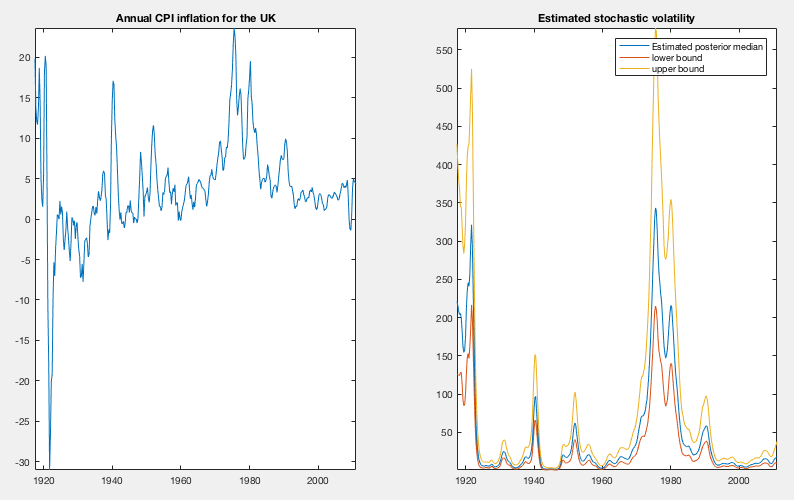
\includegraphics[height=6cm]{svol-cpi-inflation.png}
  \end{center}
  % Beobachtungsgleichung nicht linear => Algorithmus von Carter und Kohn kann nicht angewandt werden
\end{frame}

\subsection{Bayessche Inferenz (mit unabhängigem MH)}

\begin{frame}[t]
  \frametitle{Bayessche Inferenz im stochastischen Volatilitätsmodell}

  \begin{modelbox}
    \[
      \arraycolsep=2.5pt
      \begin{array}{rclll}
        y_t &=& \epsilon_t \sqrt{\stepOne{h_t}}, & \epsilon_t \sim \Normal(0, 1), & \typeInfo{t = 1, \ldots, T} \\
        \ln \stepOne{h_t} &=& \ln \stepOne{h_{t-1}} + v_t, & v_t \sim \Normal(0, \stepTwo{g}), & \typeInfo{t = 1, \ldots, T}
      \end{array}
    \]
  \end{modelbox}

  \begin{onlyenv}<1->
    Wir erfinden eine weitere Volatilitätsvariable $h_0$ hinzu.
    Diese habe die Prior-Verteilung $h_0 \sim \Normal(\overline{\mu}, \overline{\sigma}^2)$.
    \only<2->{Für die Full-Conditional-Verteilung gilt:}
    \[
      \arraycolsep=1.5pt
      \begin{array}{rcl}
        \only<2->{
          f(h_0 \,|\, h_{-0}, g, \vec{y})
        }
        \only<-7>{
          \only<2->{
            &=& f(h_0 \,|\, h_1, g)
          } \\
          \only<3->{
            &\propto& f(h_0) \cdot f(h_1 \,|\, h_0, g)
          } \\
          \visible<5->{
            &\propto& \tfrac{1}{\sqrt{\overline{\sigma}^2}} \exp \left( \tfrac{- (\ln h_0 - \overline{\mu})^2}{2 \overline{\sigma}^2} \right) \cdot \tfrac{1}{h_0} \exp \left( \tfrac{- (\ln h_1 - \ln h_0)^2}{2 g} \right)
          } \\
        }
        \only<6-8>{
          &\propto&
          \only<8>{\hphantom{\tfrac{1}{\sqrt{2 \pi \sigma_0^2}}}}
          \tfrac{1}{h_0} \exp \left( \tfrac{- (\ln h_0 - \mu_0)^2}{2 \sigma_0} \right)
        }
        \only<9->{
          &=& \tfrac{1}{\sqrt{2 \pi \sigma_0^2}} \tfrac{1}{h_0} \exp \left( \tfrac{- (\ln h_0 - \mu_0)^2}{2 \sigma_0^2} \right)
        } \\
        \visible<6->{
          && \text{mit } \sigma_0^2 \!\coloneqq\! \tfrac{\overline{\sigma}^2 g}{\overline{\sigma}^2 + g}, \enspace \mu_0 \!\coloneqq\! \sigma_0^2 \left( \tfrac{\overline{\mu}}{\overline{\sigma}^2} + \tfrac{\ln h_1}{g} \right)
        }
      \end{array}
    \]
  \end{onlyenv}
  \begin{onlyenv}<4-6>
    \begin{nebenrechnung}
      \[
        \arraycolsep=2.5pt
        \begin{array}{rcll}
          f(h_{s+1} \,|\, h_s) &=& \tfrac{1}{\sqrt{2 \pi g}} \tfrac{1}{h_{s+1}} \exp \left( \tfrac{- (\ln h_{s+1} - \ln h_s)^2}{2 g} \right) & \qquad \text{\typeInfo{(Log. Normalvert.)}}
        \end{array}
      \]
    \end{nebenrechnung}
  \end{onlyenv}

  \begin{onlyenv}<10->
    Für die Zeitpunkte $t = 1,, \ldots T{-}1$ gilt:
    \[
      \arraycolsep=2.5pt
      \begin{array}{rcl}
        f(h_t \,|\, h_{-t}, \vec{y}, g)
        \only<-14>{
          &=& f(h_t \,|\, h_{t-1}, h_{t+1}, y_t, g) \\
          \visible<11->{
            &\propto& f(y_t \,|\, h_t, g) \cdot f(h_{t+1} \,|\, h_t, g) \cdot f(h_t \,|\, h_{t-1}, g)
          } \\
        }
        \visible<13->{
          &\propto& \tfrac{1}{\sqrt{h_t}} \exp \left( - \tfrac{y_t^2}{2 h_t} \right) \cdot \tfrac{1}{h_t} \exp \left( - \tfrac{(\ln h_t - \mu_t)^2}{2 \sigma_t^2} \right) \\
          && \text{mit } \mu_t \coloneqq \tfrac{1}{2} (\ln h_{t+1} + \ln h_{t-1}), \quad \sigma_t^2 \coloneqq \tfrac{1}{2} g
        }
      \end{array}
    \]
  \end{onlyenv}
  \begin{onlyenv}<12-13>
    \begin{nebenrechnung}
      \[
        \arraycolsep=2.5pt
        \begin{array}{rcll}
          f(y_t \,|\, h_t) &=& \tfrac{1}{\sqrt{2 \pi h_t}} \exp \left( \tfrac{- y_t^2}{2 h_t} \right) & \qquad \text{\typeInfo{(Normalverteilung)}}
          % \\ f(h_{s+1} \,|\, h_s) &=& \tfrac{1}{\sqrt{2 \pi}} \tfrac{1}{h_{s+1}} \exp \left( \tfrac{- (\ln h_{s+1} - \ln h_s)^2}{2 g} \right) & \qquad \text{\typeInfo{(Log. Normalvert.)}}
        \end{array}
      \]
    \end{nebenrechnung}
  \end{onlyenv}

  \begin{onlyenv}<16->
    Für die letzte Volatilitätsvariable $h_T$ gilt
    \[
      \arraycolsep=2.5pt
      \begin{array}{rcl}
        f(h_T \,|\, h_{-T}, \vec{y}, g)
        \only<-18>{
          &=& f(h_T, h_{T-1}, y_T, g) \\
          \visible<17->{
            &\propto& f(y_T \,|\, h_t) \cdot f(h_T \,|\, h_{T-1}) \\
          }
        }
        \visible<18->{
          &\propto& \tfrac{1}{\sqrt{h_T}} \exp \left( - \tfrac{y_T^2}{2 h_T} \right) \cdot \tfrac{1}{h_T} \exp \left( \tfrac{- (\ln h_T - \mu_T)^2}{2 \sigma_T^2} \right) \\
          && \text{mit } \mu_T \coloneqq \ln h_{T-1}, \quad \sigma_T^2 \coloneqq g
        }
      \end{array}
    \]
    \only<19>{\,}
  \end{onlyenv}
\end{frame}

\begin{frame}[t]
  \frametitle{Bayessche Inferenz im stochastischen Volatilitätsmodell}
  \begin{enumerate}
    \item<2->[A.] Setze die Parameter der Prior-Vert. $h_0 \sim \Normal(\overline{\mu}, \overline{\sigma}^2)$ sowie $g \sim \InverseGamma(\tfrac{g_0}{2}, \tfrac{\nu_0}{2})$
    \item<3->[B.] Initialisierung: Wähle Startwerte für $h_0, \ldots, h_T$ und $g$
    \item<4->[C.] Gibbs-Sampling: Wiederhole die Schritte
    \begin{enumerate}
      \item<5->[\stepOne{1.}] Führe einen Metropolis-Hastings-Schritt für \stepOne{$h_0, \ldots, h_T$} aus:
      \begin{itemize}
        \item<6-> Ziehe $h_0$ neu aus der logarithmischen Normalverteilung
        \[
          f(h_0 \,|\, h_1, g) = \tfrac{1}{\sqrt{2 \pi \sigma_0^2}} \tfrac{1}{h_0} \exp \left( \tfrac{- (\ln h_0 - \mu_0)^2}{2 \sigma_0^2} \right), \enspace
          \sigma_0^2 \coloneqq \tfrac{\overline{\sigma} g}{\overline{\sigma}^2 + g}, \enspace
          \mu_0 \coloneqq \sigma_0^2 \left( \tfrac{\overline{\mu}}{\overline{\sigma}^2} + \tfrac{\ln h_1}{g} \right)
        \]
        \item<7-> Für $t = 1, \ldots, T$ ziehe einen Kandidaten $h_{t, \new}$ gemäß der log. Normalverteilung
        \[
          q(h_{t,\new}) = \tfrac{1}{\sqrt{2 \pi \sigma_t^2}} \tfrac{1}{h_{t, \new}} \exp \left( \tfrac{- (\ln h_{t, \new} - \mu_t)^2}{2 \sigma_t^2} \right)
        \]
        mit $\mu_t$ und $\sigma_t$ wie auf der letzten Folie.

        Berechne die Akzeptanz-Wahrscheinlichkeit $\alpha = \min(1, r)$ mit
        \[
          r \coloneqq \frac{h_{t,\new}^{-0,5} \exp \left( \nicefrac{-y_t^2}{2 h_{t, \new}} \right)}{h_{t,\old}^{-0,5} \exp \left( \nicefrac{-y_t^2}{2 h_{t, \old}} \right)}
        \]
        Ziehe $u \sim \Uniform(0,1)$. Akzeptiere $h_{t, \new}$, falls $u < \alpha$, ansonsten behalte $h_{t, \old}$.
      \end{itemize}
      \item<8->[\stepTwo{2.}] Sample \stepTwo{$g$} geg. \stepOne{$h_0, \ldots, h_T$}:
      Ziehe ein neues~$g$ aus der Full-Cond.-Verteilung $\InverseGamma(\tfrac{\tilde{g}}{2}, \tfrac{\tilde{\nu}}{2})$ mit $\tilde{g} \coloneqq g_0 + \sum_{t=1}^T v_t = g_0 + \sum_{t=1}^T \ln h_t - \ln h_{t-1}$ und $\tilde{\nu} \coloneqq \nu_0 + T$.
    \end{enumerate}
  \end{enumerate}
\end{frame}

\section[Erweitertes stoch. Volatilitätsmodell]{Erweiterte Version des stochastischen Volatilitätsmodells}

\begin{frame}
  \frametitle{Erweiterte Version des stochastischen Volatilitätsmodells}
  \begin{modelbox}
    \[
      \arraycolsep=3pt
      \begin{array}{rclll}
        y_t &=& \stepThree{c_t} + \stepThree{b_t} y_{t-1} + \epsilon_t \sqrt{\stepOne{h_t}}, & \enspace \epsilon_t \sim \Normal(0, 1), & \quad \typeInfo{t = 1, \ldots, T} \\
        \ln \stepOne{h_t} &=& \ln \stepOne{h_{t-1}} + v_t, & \enspace v_t \sim \Normal(0, \stepTwo{g}), \\
        \stepThree{B_t} &=& \stepThree{B_{t-1}} + e_t, & \enspace e_t \sim \Normal(0, \stepThree{Q}), & \quad \typeInfo{Q \in \R^{2 \times 2}}
      \end{array}
    \]
  \end{modelbox}
  Dabei ist $\stepThree{B_t = \begin{psmallmatrix} c_t \\ b_t \end{psmallmatrix}} \typeInfo{\,\in \R^2}$ der Vektor der AR-Koeffizienten.
\end{frame}

\subsection{Bayessche Inferenz (mit unabhängigem MH)}

\begin{frame}[t]
  \frametitle{Bayessche Inferenz im erweiterten stoch. Volatilitätsmodell}

  \begin{modelbox}
    \[
      \arraycolsep=3pt
      \begin{array}{rclll}
        y_t &=& \stepThree{c_t} + \stepThree{b_t} y_{t-1} + \epsilon_t \sqrt{\stepOne{h_t}}, & \enspace \epsilon_t \sim \Normal(0, 1), & \quad \typeInfo{t = 1, \ldots, T} \\
        \ln \stepOne{h_t} &=& \ln \stepOne{h_{t-1}} + v_t, & \enspace v_t \sim \Normal(0, \stepTwo{g}), \\
        \stepThree{B_t} &=& \stepThree{B_{t-1}} + e_t, & \enspace e_t \sim \Normal(0, \stepThree{Q}), & \quad \typeInfo{Q \in \R^{2 \times 2}}
      \end{array}
    \]
  \end{modelbox}

  \begin{enumerate}
    \item<2->[A.] Setze die Parameter der Prior-Verteilung:
    \[
      g \sim \InverseGamma(\tfrac{g_0}{2}, \tfrac{\nu_0}{2}), \quad
      Q \sim \InverseWishart(Q_0, T_0), \quad
      h_0 \sim \Normal(\overline{\mu}, \overline{\sigma}^2)
    \]
    \item<3->[B.] Initialisierung: Wähle Startwerte für $h_0, \ldots, h_T$, $g$, $B_1, \ldots, B_T$ und $Q$ \\
    (benutze dazu Training-Daten)
    \item<4->[C.] Gibbs-Sampling: Wiederhole die Schritte
    \begin{enumerate}
      \item<5->[\stepOne{1.}] Aktualisiere \stepOne{$h_0$, \ldots, $h_T$} gegeben~\stepTwo{$g$} und \stepThree{$B_1, \ldots B_T$}:
      \begin{itemize}
        \item<6-> Ziehe~$h_0$ neu (genau wie beim letzten Modell)
        \item<7-> Für $t = 1, \ldots, T$ führe einen MH-Schritt für $h_t$ aus.
        Die Details sind wie beim letzten Schritt mit dem einzigen Unterschied, dass jetzt $y_t - c_t - b_t y_{t-1} \sim \Normal(0, h_t)$ gilt (anstatt $y_t \sim \Normal(0, h_t)$).
      \end{itemize}
      \item<8->[\stepTwo{2.}] Ziehe \stepTwo{$g$} neu gegeben \stepOne{$h_0, \ldots, h_T$} (genau wie bisher)
      \item<9->[\stepThree{3.}] Aktualisiere \stepThree{$B_1, \ldots, B_T$} und \stepThree{$Q$} gegeben \stepOne{$h_0, \ldots, h_T$} und \stepTwo{$g$}
      \begin{itemize}
        \item<10-> Führe einen MH-Schritt für \stepThree{$B_1, \ldots, B_T$} aus wie im letzten Vortrag (einziger Unterschied: Varianz hängt jetzt von $t$ ab).
        \item<11-> Ziehe ein neues $Q$ aus seiner Full-Conditional-Verteilung $\InverseWishart(\tilde{S}, \tilde{T})$ mit $\tilde{S} = Q_0 + \sum_{t=1}^T (B_t - B_{t-1})^T (B_t - B_{t-1})$ und $\tilde{T} = T_0 + T$.
      \end{itemize}
    \end{enumerate}
  \end{enumerate}
\end{frame}

\end{document}
